\documentclass{article}
\usepackage{amsmath}
\usepackage{graphics}
\usepackage{hyperref}
\usepackage{cite}
\usepackage[pdftex]{graphicx} % with the driver option
\title{Hybrid radiopropa ray tracer}
\author{Arthur Adriaens}
\date{\today}

\begin{document}
	\maketitle
\section{random number generator}
We'll use the numpy random module to generate the random numbers, the
considered square (as there is only a z component to the ice model the 3D
problem is essentially only a 2D problem) is x:-4km,+4km and z:0,-3km. A good
test to see if the generator is both random and uniform is to plot the next
element to the previous element, shown in figure \ref{fig:randomnumberz} for
the generated z coordinates,
in figure \ref{fig:randomnumberx} for the generated x coordinates.
This clearly is a good random number generator and is the one we'll be using
for the testing of the hybrid ray tracer.  As a counter-example, a bad random
number generator's expected output is shown in figure \ref{fig:badrandom}

\begin{figure}[ht]
  \centering
  \begin{minipage}[b]{0.49\textwidth}
    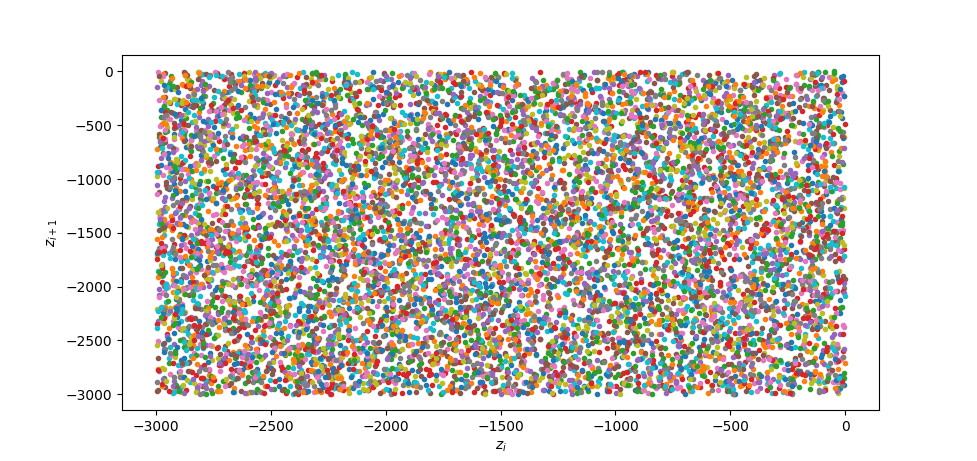
\includegraphics[width=\textwidth]{figures/randomnumberz.png}
    \caption{$z_{i+1}$ i.f.o $z_i$}
    \label{fig:randomnumberz}
  \end{minipage}
  \hfill
  \begin{minipage}[b]{0.49\textwidth}
    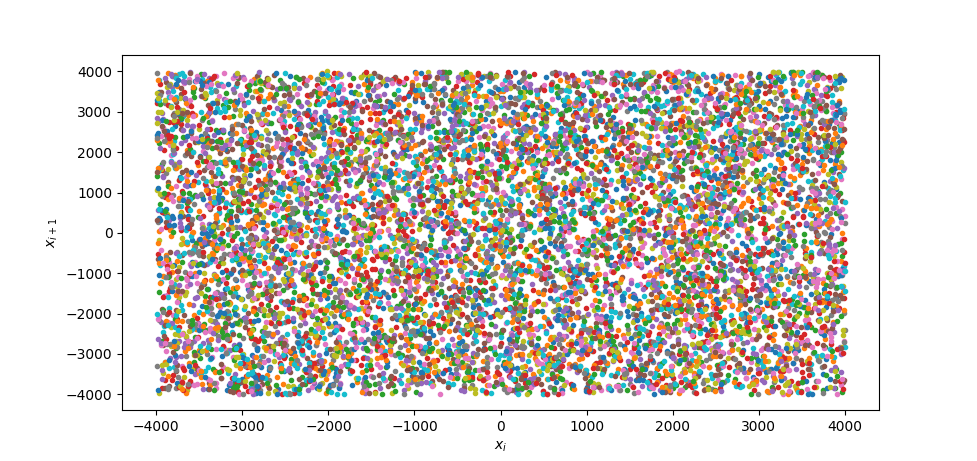
\includegraphics[width=\textwidth]{figures/randomnumberx.png}
    \caption{$x_{i+1}$ i.f.o $x_i$}
    \label{fig:randomnumberx}
  \end{minipage}
\end{figure}

\begin{figure}[ht]
	\centering
	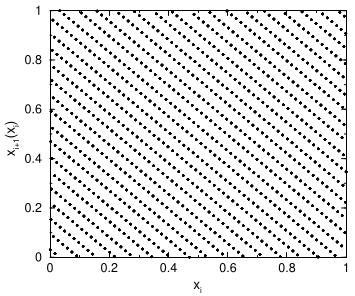
\includegraphics[width=0.4\textwidth]{figures/BadRandom.png}
	\caption{bad random number generator}
	\label{fig:badrandom}
\end{figure}
\newpage
\section{How it works}
\begin{figure}[ht]
	\centering
	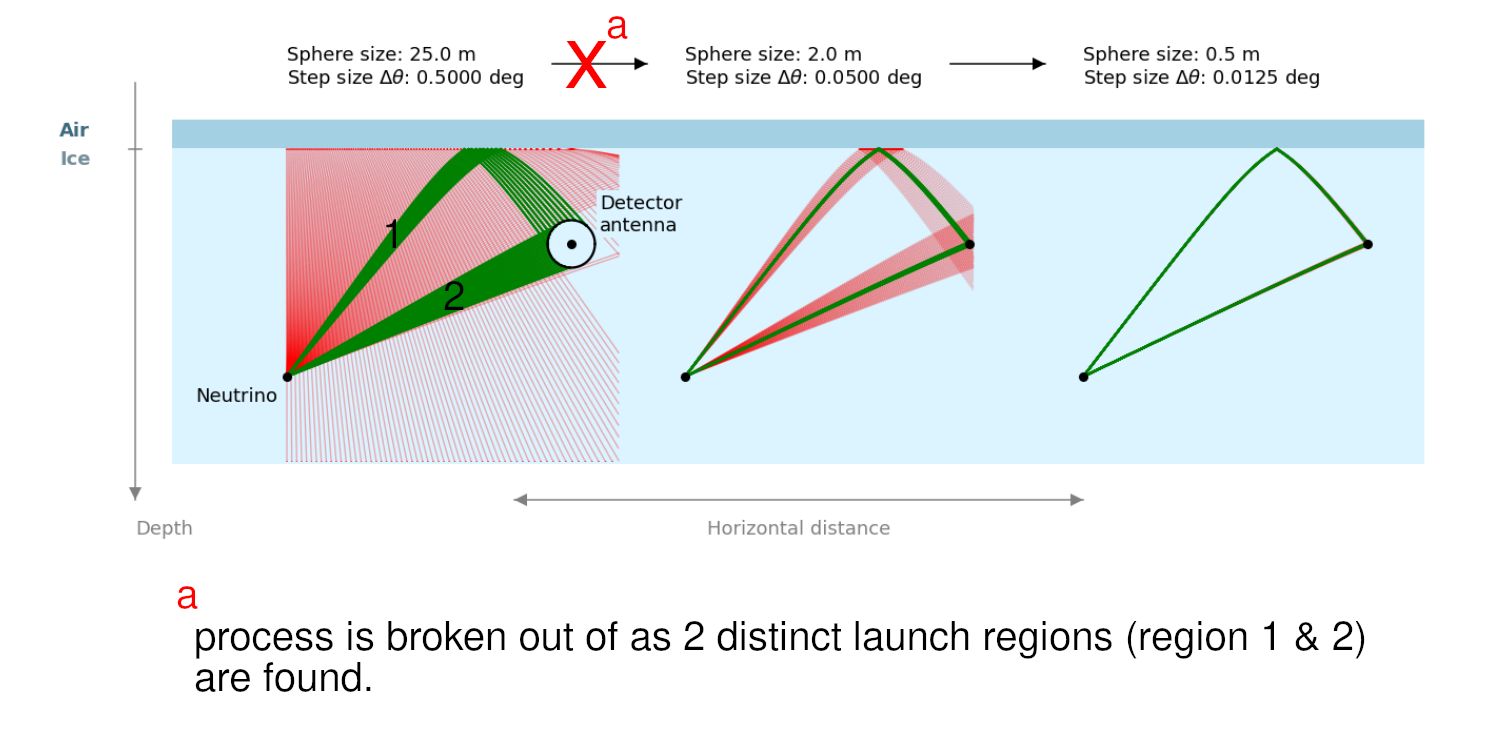
\includegraphics[width=\textwidth]{figures/explanation.png}
	\caption{explanation of the hybrid method}
	\label{fig:explanation}
\end{figure}
The hybrid minimizer can be seen as an extension of the iterative minimizer, it
checks after the first loop (as explained in the paper by B. Oeyen et al.
\cite{2022icrc.confE1027O}) if there are 2 distinct launch regions, if this is
the case it breaks out of the loop and uses the scipy.optimize.minimize module
to find the solutions in the respective angle intervals. If it doesn't find 2 distinct regions after the first loop, it checks again the next loop. This is visually explained using 
a modified version of B. Oeyen et al. their figure in figure \ref{fig:explanation}. 
\section{performance}
\subsection{speed}
I did a test with 10000 coordinates who were randomly generated (as
mentioned above) and each ray tracer was used on these 10000 coordinates,
checking the time it took per solution to check the speed of this algorithm and
compare it with the iterative ray tracer. It turns out that on average we get
(for my HP ProBook with an i5-6200U at 2.8GHz):
\begin{itemize}
	\item a hybrid solution time of 7.69 seconds
	\item an iterative solution time of 1.538 seconds
\end{itemize}
So it takes $\approx$ 5 times as long.
\subsection{accuracy}
Now happily it's not just slower, it's actually a more accurate ray tracer:
%----------------------------------------------------------------------------------------
%       REFERENCE LIST
%----------------------------------------------------------------------------------------
\bibliography{sources}
\bibliographystyle{plain}

\end{document}

